\chapter{Les étapes d'une approche data-driven}
\chapterintrobox{Une approche de pronostic \acrlong{dd} (une approche qui s’appuie sur des données opérationnelles historiques pour construire un modèle qui est utilisé pour prédire la durée de vie utile restante) doit passer par de multiples étapes—de l’acquisition de données jusqu’à l’estimation de la durée de vie utile restante. Dans ce chapitre, ces différentes étapes seront examinées en détail.}

\section{Aquisition de données}
\label{sec:data-acquisition}
Un signal est une fonction qui transmet des informations sur le comportement d'un système ou les attributs d'un phénomène. les signaux se produisent naturellement et sont également synthétisés. Un signal n'est pas nécessairement une grandeur électrique. Cependant, pour effectuer des activités telles que la synthèse, le transport, l'enregistrement, l'analyse et la modification de signaux, il est souvent pratique d'utiliser un signal sous la forme d'une grandeur électrique \cite{Priemer1990}.

L'acquisition de données est un processus de capture et de stockage de différents types de données de surveillance (signaux) provenant de divers capteurs installés sur l'équipement surveillé. C'est le premier processus de pronostic des machines, qui fournit des informations de base de surveillance d'état (\acrlong{cm}) pour les processus suivants. Un système d'acquisition de données est composé de capteurs, de dispositifs de transmission de données et de dispositifs de stockage de données \cite{Lei2018}. Les données de surveillance d'état sont très versatiles. Il peut s'agir de données sur les vibrations, de données acoustiques, de données d'analyse d'huile, de données sur la température, la pression, l'humidité, les conditions météorologiques ou l'environnement, etc. Les différents capteurs, tels que les micro-capteurs, les capteurs à ultrasons et les capteurs d'émission acoustique ont été conçus pour collecter différents types de données. Les technologies sans fil, telles que Bluetooth, ont fourni une solution alternative à la communication de données à un prix avantageux \cite{Jardine2006}.

Bien que la recherche sur des concepts avancés comme les réseaux de capteurs sans fil et la récolte d’énergie pour alimenter des capteurs autonomes soit en cours, l’acquisition de données (capteurs) et la manipulation sont aujourd’hui plutôt bien établies. Par conséquent, une grande partie de la recherche dans cette discipline se concentre sur l’analyse des données obtenues pour en extraire de l’information \cite{Tinga2014}. Parce que cette discipline est bien développée, beaucoup de nouvelles installations et techniques d’acquisition de données ont été conçues et appliquées dans les industries modernes. Ces installations puissantes et polyvalentes ont rendu l’acquisition de données pour la mise en œuvre du PHM plus pratique et plus faisable \cite{Lei2016}.

\section{Extraction de Caractéristiques}
L'approche de pronostic data-driven est principalement utilisée lorsqu'il est difficile de comprendre le comportement physique d'un système complexe. La compréhension du comportement et de l'interaction des différents éléments qui conduisent à la dégradation des machines est le point de départ pour développer un modèle physique pour les pronostics.
D'autre part, cette approche utilise des données de surveillance des conditions pour modéliser implicitement son comportement. Les modèles utilisés dans l'approche data-driven utilisent des données de surveillance pour modéliser un comportement complexe et capturer des modèles complexes, mais ils sont considérés comme des boîtes noires : ils ne fournissent pas nécessairement un aperçu du processus.
En général, la performance de ces modèles dépend de la qualité des données d'entrée (données). La partie humaine ne peut pas effectuer la tâche que le modèle effectue, mais le traitement des données d'entrée peut augmenter considérablement les résultats. Ce traitement est nécessaire parce que les données des capteurs sur lesquelles le modèle repose sont généralement redondantes, bruyantes et incomplètes, ces imperfections sont dues à de nombreuses raisons.

L'extraction de caractéristiques est une étape de prétraitement importante dans le processus de développement des modèles d'apprentissage machine et influence directement les performances du modèle. Par conséquent, cette étape doit être réalisée avec soin afin d'extraire des caractéristiques significatives des données brutes. Les données sur les vibrations contiennent des informations très utiles sur l'état du système, mais elles nécessitent un prétraitement important avant d'être utilisées comme données d'entrée pour un modèle spécifique. Ce chapitre décrit certaines des techniques de traitement du signal utilisées dans l'analyse vibratoire traditionnelle, mais dans ce contexte, elles seront utilisées comme extracteurs de caractéristiques pour une architecture de réseau de neurones.

\subsection{Traitement du signal}
Le traitement du signal est l'étude et l'analyse des signaux stockés afin de révéler leurs propriétés—qui peuvent ne pas être apparentes au premier abord, en utilisant un ensemble d'algorithmes et de techniques. Dans le contexte de la surveillance de l'état, ces propriétés révélées par le traitement du signal peuvent être révélatrices de santé de la machine.
Le traitement du signal est un sous-domaine bien établi et mature du génie électrique, avec de nombreuses techniques et algorithmes proposés dans la littérature.


Le traitement du signal peut être classé en trois catégories : \textbf{Analyse Temporelle}, \textbf{Analyse Fréquentielle} et \textbf{Analyse Temps–Fréquence}.

\subsubsection{Analyse Temporelle}
Les mesures originales des signaux qui sont généralement échantillonnés de manière répétée entre des intervalles de temps prédéfinis sont sous forme de domaine temporel. Ainsi, l'analyse du domaine temporel est directement basée sur la mesure originale \cite{Lei2016}.


\subsubsection{Analyse Fréquentielle}
L'analyse du domaine fréquentiel est basée sur les signaux transformés dans le domaine fréquentiel. L'avantage de l'analyse en domaine fréquentiel par rapport à l'analyse en domaine temporel est sa capacité à décomposer les signaux originaux en une série de composantes fréquentielles. L'analyse du domaine fréquentiel la plus utilisée est l'analyse du spectre au moyen de la transformée de Fourier rapide (FFT). L'idée principale de l'analyse spectrale est d'isoler et de localiser certaines composantes de fréquence d'intérêt relatives aux caractéristiques de défaut des machines \cite{Lei2016a}.


\subsubsection{Analyse Temps–Fréquence}
Le problème de l'analyse du domaine temporel et de l'analyse du domaine fréquentiel est que chacune d'elles ne dispose d'aucune information sur l'autre domaine (l'analyse du domaine temporel ne dispose d'aucune information sur le domaine fréquentiel, et l'analyse du domaine fréquentiel ne dispose d'aucune information sur la position dans le temps).

Ainsi, l'analyse du domaine temps-fréquence, qui
étudie les signaux de mesure dans les domaines du temps et des fréquences, a été appliquée à l'analyse des signaux de mesure non stationnaires. L'analyse temps-fréquence décrit les caractéristiques des signaux de mesure dans les fonctions bidimensionnelles du temps et de la fréquence afin de mieux révéler les modes de défaillance des machines.


La figure \ref{fig:signal-processing} présente les différentes techniques utilisées pour chaque type d'analyse:

\begin{figure}[h]
    \centering
	\begin{tikzpicture}
\tikzstyle{element}=[draw,rectangle]
\tikzstyle{entity}=[fill=gray!20,align=center, text width=8em]
\node[element] (fe) {Signal processing};


\node[element,below = 1.6em of fe] (fd) {Frequency analysis};
\node[element,left = of fd] (td) {Time series analysis};
\node[element,right = of fd] (tfd) {Time--Frequency analysis};

\node[entity,below =.5em of td] (stat) {Statistics-based};
\node[entity,below =.5em of stat] (arm) {Autoregressive Model};
\node[entity,below =.5em of arm] (arma) {ARMA Model};
\node[entity,below =.5em of arma] (tsa) {Time Synchronous Average};

\node[entity,below =.5em of fd] (fft) {Fourier Transform};
\node[entity,below =.5em of fft] (cep) {Cepstrum};
\node[entity,below =.5em of cep] (hil) {Hilbert Transform};\node[entity,below =.5em of hil] (env) {Envelope Analysis};


\node[entity,below =.5em of tfd] (stft) {Short-Time Fourier Transform};
\node[entity,below =.5em of stft] (wt) {Wavelet Transform};
\node[entity,below =.5em of wt] (hht) {Hilbert-Huang Transform};
\node[entity,below =.5em of hht,align=center, text width=8em] (emd) {Empirical Mode Decomposition};

\draw[->,>=angle 60] (fe.south) -- ++(0,0) -- ++(0,-.8em) -| (td);
\draw[->,>=angle 60] (fe.south) -| (fd);
\draw[->,>=angle 60] (fe.south) -- ++(0,0) -- ++(0,-.8em) -| (tfd);
\end{tikzpicture}

    \caption{Techniques de traitement du signal dans les différents domaines}
    \label{fig:signal-processing}
\end{figure}


\subsection{Analyse de Fourier}
L'analyse de Fourier, également appelée analyse harmonique, d'un signal périodique $x(t)$ est la décomposition de la série en sommation de composantes sinusoïdales, où chaque sinusoïde a une amplitude et une phase spécifiques.

La transformation de Fourier (FT) d'un signal $x(t)$ peut être mathématiquement donnée par l'équation \ref{equation:fourier-transform} :

\begin{equation}
    X(w) = \int_{-\infty}^{\infty}x(n)e^{-jwt}dt
    \label{equation:fourier-transform}
\end{equation}

Dans les applications pratiques du traitement numérique des signaux où les signaux sont discrets dans le temps plutôt que continus (par exemple l'analyse des vibrations), on utilise plutôt une version discrétisée appelée transformation de Fourier discrète (TFD), qui est exprimée mathématiquement par l'équation \ref{equation:discrete-fourier-transform} :

\begin{equation}
    X(w) = \sum_{-\infty}^{\infty}x(t)e^{-jwt}dt
    \label{equation:discrete-fourier-transform}
\end{equation}

La Fast Fourier Transform (FFT) est un algorithme efficace utilisé pour implémenter la TFD dans les ordinateurs. La figure \ref{figure:fft} montre un signal dans sa forme d'onde (ou domaine temporel) et son spectre correspondant (domaine fréquentiel) obtenu à l'aide de l'algorithme FFT. Le spectre montre les composantes de fréquence présentes dans le signal:

\begin{figure}[h]
    \centering
    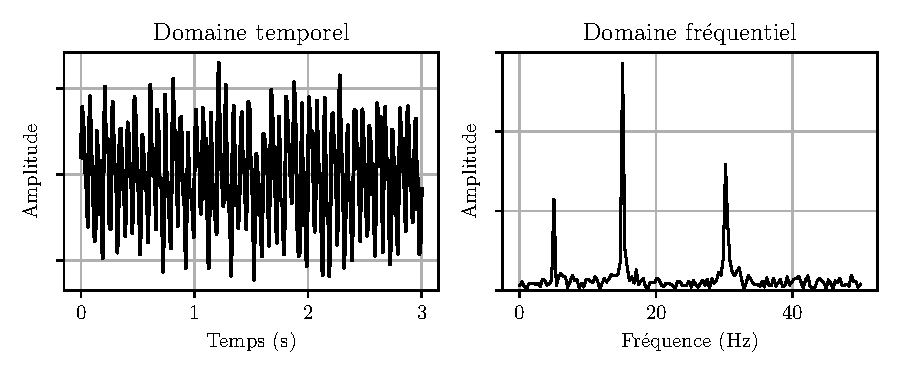
\includegraphics{figures/fft_fr.pdf}
    \caption{Signal dans le domaine temporel et sa transformation de Fourier rapide}
    \label{figure:fft}
\end{figure}


\subsection{Transformation en Ondelettes}
La transformation en ondelettes est également un outil d'analyse spectrale, comme la transformation de Fourier. La principale différence est que la transformation de Fourier décompose le signal en composantes sinusoïdales, mais que la transformation en ondelettes le décompose en un ensemble de fonctions oscillatoires appelées \textbf{ondelettes}. Contrairement aux sinusoïdes, les ondelettes sont localisées dans le temps, ainsi la transformation en ondelettes ne fournit pas seulement des informations sur la fréquence présente dans un signal mais aussi sur le moment de leur apparition. La transformation en ondelettes est une bien meilleure solution que la transformation de Fourier lorsqu'on étudie des signaux non linéaires et non stationnaires (c'est-à-dire que ses composantes de fréquence varient avec le temps).

La figure \ref{fig:time-frequency-plane} montre la différence de résolution en temps et en fréquence entre les différentes méthodes. Dans la forme d'onde, le signal a une résolution absolue en temps et une résolution nulle en fréquence. La transformation de Fourier, au contraire, transforme totalement le signal dans le domaine fréquentiel, ce qui lui confère une résolution absolue en fréquence mais aucune résolution en temps. La transformation de Fourier à court terme est calculée à l'identique à la transformation de Fourier, mais elle est effectuée sur des segments séparés du signal original afin de préserver une certaine résolution dans le temps. La transformation en ondelettes présente une résolution temporelle élevée pour les hautes fréquences et une résolution haute fréquence pour les basses fréquences.

\begin{figure}[H]
    \centering
    \begin{subfigure}{.35\textwidth}
	\centering
	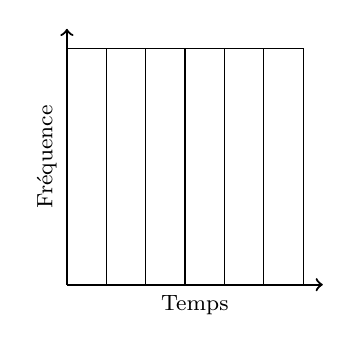
\begin{tikzpicture}
	\draw (0,0) -- (3,0);
	\draw (3,0) -- (3,-3);
	\path[thick, ->]  (0,-3) edge node[below] {\footnotesize Temps} (3.25,-3)  ;
	\path[thick, ->] (0,-3) edge node[above, rotate=90] {\footnotesize Fréquence} (0,.25)  ;
	
	\draw (.5,0) -- (.5,-3);
	\draw (1,0) -- (1,-3);
	\draw (1.5,0) -- (1.5,-3);
	\draw (2,0) -- (2,-3);
	\draw (2.5,0) -- (2.5,-3);
	
	\draw (3,0) -- (3,-3);
	\end{tikzpicture}
	\caption{Forme d'onde}
\end{subfigure}%
\begin{subfigure}{.35\textwidth}
	\centering
	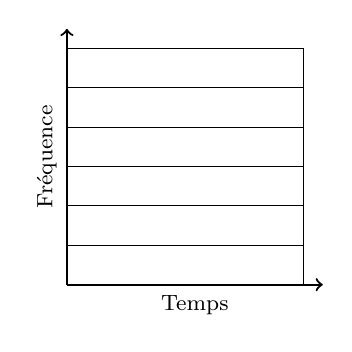
\begin{tikzpicture}
	\draw (0,0) -- (3,0);
	\draw (3,0) -- (3,-3);
	\path[thick, ->]  (0,-3) edge node[below] {\footnotesize Temps} (3.25,-3)  ;
	\path[thick, ->] (0,-3) edge node[above, rotate=90] {\footnotesize Fréquence} (0,.25)  ;
	
	\draw (0,-.5) -- (3,-.5);
	\draw (0,-1) -- (3,-1);
	\draw (0,-1.5) -- (3,-1.5);
	\draw (0,-2) -- (3,-2);
	\draw (0,-2.5) -- (3,-2.5);
	
	\end{tikzpicture}
	\caption{Transformation de Fourier}
\end{subfigure}

\medskip

\begin{subfigure}{.35\textwidth}
	\centering
	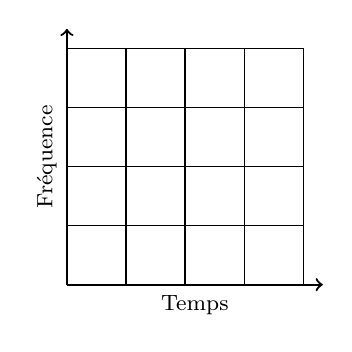
\begin{tikzpicture}
	
	\draw (0,0) -- (3,0);
	\draw (3,0) -- (3,-3);
	\path[thick, ->]  (0,-3) edge node[below] {\footnotesize Temps} (3.25,-3)  ;
	\path[thick, ->] (0,-3) edge node[above, rotate=90] {\footnotesize Fréquence} (0,.25)  ;
	
	\draw (0.75,0) -- (0.75,-3);
	\draw (0,-0.75) -- (3,-0.75);
	\draw (1.5,0) -- (1.5,-3);
	\draw (2.25,0) -- (2.25,-3);
	\draw (0,-1.5) -- (3,-1.5);
	%	\draw (3,0) -- (3,-3);
	\draw (0,-2.25) -- (3,-2.25);
	
	\end{tikzpicture}
	\caption{Fourier à court terme}
\end{subfigure}%
\begin{subfigure}{.35\textwidth}
	\centering
	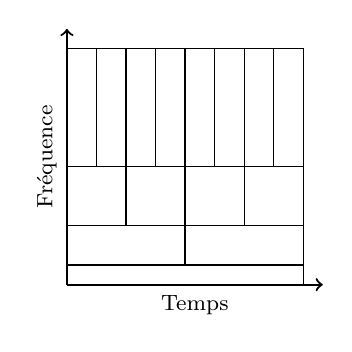
\begin{tikzpicture}
	\draw (0,0) -- (3,0);
	\draw (3,0) -- (3,-3);
	\path[thick, ->]  (0,-3) edge node[below] {\footnotesize Temps} (3.25,-3)  ;
	\path[thick, ->] (0,-3) edge node[above, rotate=90] {\footnotesize Fréquence} (0,.25)  ;
	\draw (0,-1.5) -- (3,-1.5);
	\draw (0,-2.25) -- (3,-2.25);
	
	\draw (0,-2.75) -- (3,-2.75);
	\draw (1.5,0) -- (1.5,-2.75);
	
	\draw (0.75,0) -- (0.75,-2.25);
	\draw (2.25,0) -- (2.25,-2.25);
	
	\draw (0.375,0) -- (0.375,-1.5);
	\draw (1.125,0) -- (1.125,-1.5);
	\draw (1.875,0) -- (1.875,-1.5);
	\draw (2.625,0) -- (2.625,-1.5);
	\end{tikzpicture}
	\caption{Transformation en ondelettes}
\end{subfigure}


\begin{comment}
%BIGGER VERSION

\begin{subfigure}{.4\textwidth}
	\centering
	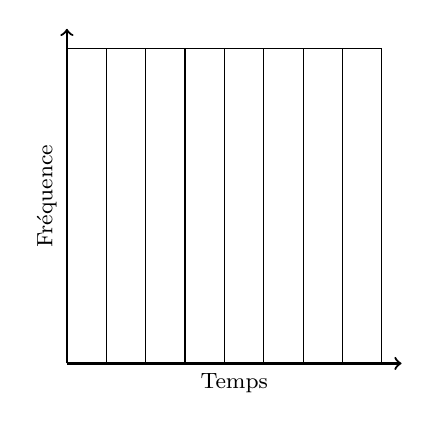
\begin{tikzpicture}
	\draw (0,0) -- (4,0);
	\draw (4,0) -- (4,-4);
	\path[thick, ->]  (0,-4) edge node[below] {\footnotesize Temps} (4.25,-4)  ;
	\path[thick, ->] (0,-4) edge node[above, rotate=90] {\footnotesize Fréquence} (0,.25)  ;
	
	\draw (.5,0) -- (.5,-4);
	\draw (1,0) -- (1,-4);
	\draw (1.5,0) -- (1.5,-4);
	\draw (2,0) -- (2,-4);
	\draw (2.5,0) -- (2.5,-4);
	\draw (3,0) -- (3,-4);
	\draw (3.5,0) -- (3.5,-4);
	\end{tikzpicture}
	\caption{Waveform}
\end{subfigure}%
\begin{subfigure}{.4\textwidth}
	\centering
	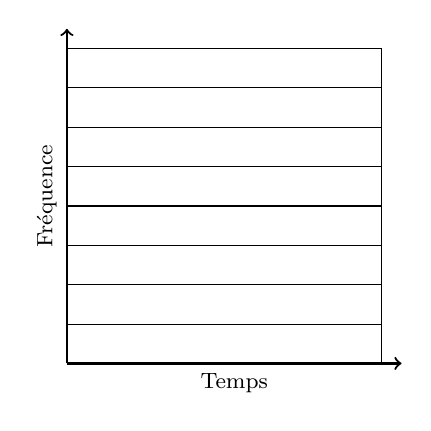
\begin{tikzpicture}
	\draw (0,0) -- (4,0);
	\draw (4,0) -- (4,-4);
	\path[thick, ->]  (0,-4) edge node[below] {\footnotesize Temps} (4.25,-4)  ;
	\path[thick, ->] (0,-4) edge node[above, rotate=90] {\footnotesize Fréquence} (0,.25)  ;
	
	\draw (0,-.5) -- (4,-.5);
	\draw (0,-1) -- (4,-1);
	\draw (0,-1.5) -- (4,-1.5);
	\draw (0,-2) -- (4,-2);
	\draw (0,-2.5) -- (4,-2.5);
	\draw (0,-3) -- (4,-3);
	\draw (0,-3.5) -- (4,-3.5);
	\end{tikzpicture}
	\caption{Fourier Transform}
\end{subfigure}

\medskip

\begin{subfigure}{.4\textwidth}
	\centering
		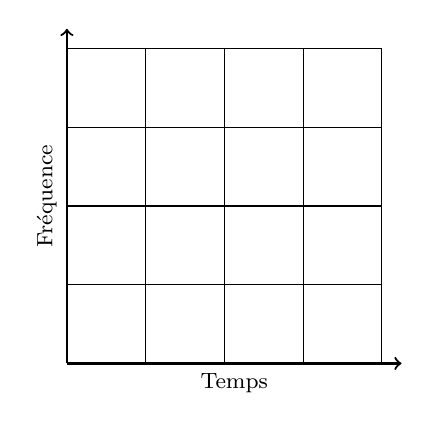
\begin{tikzpicture}
	
	\draw (0,0) -- (4,0);
	\draw (4,0) -- (4,-4);
	\path[thick, ->]  (0,-4) edge node[below] {\footnotesize Temps} (4.25,-4)  ;
	\path[thick, ->] (0,-4) edge node[above, rotate=90] {\footnotesize Fréquence} (0,.25)  ;
	
	\draw (1,0) -- (1,-4);
	\draw (0,-1) -- (4,-1);
	\draw (2,0) -- (2,-4);
	\draw (0,-2) -- (4,-2);
	\draw (3,0) -- (3,-4);
	\draw (0,-3) -- (4,-3);
	
	\end{tikzpicture}
	\caption{Short-Temps Fourier Transform}
\end{subfigure}%
\begin{subfigure}{.4\textwidth}
	\centering
	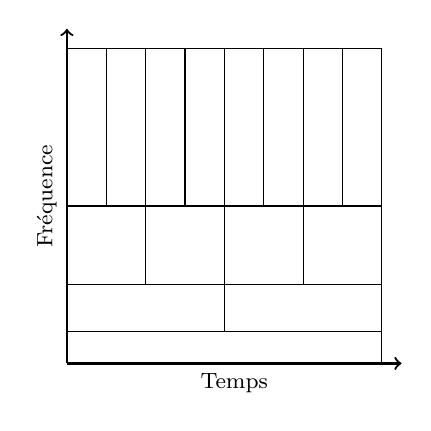
\begin{tikzpicture}
		\draw (0,0) -- (4,0);
		\draw (4,0) -- (4,-4);
		\path[thick, ->]  (0,-4) edge node[below] {\footnotesize Temps} (4.25,-4)  ;
		\path[thick, ->] (0,-4) edge node[above, rotate=90] {\footnotesize Fréquence} (0,.25)  ;
		\draw (0,-2) -- (4,-2);
		\draw (0,-3) -- (4,-3);
	
		\draw (0,-3.6) -- (4,-3.6);
		\draw (2,0) -- (2,-3.6);
	
		\draw[-] (1,0) -- (1,-3);
		\draw[-] (3,0) -- (3,-3);
	
		\draw[-] (.5,0) -- (.5,-2);
		\draw[-] (1.5,0) -- (1.5,-2);
	
		\draw[-] (2.5,0) -- (2.5,-2);
		\draw[-] (3.5,0) -- (3.5,-2);
	\end{tikzpicture}
	\caption{Wavelet Transform}
\end{subfigure}
\end{comment}

    \caption{Plan de résolution temps--fréquence}
    \label{fig:time-frequency-plane}
\end{figure}

Il existe une grande variété d'ondelettes qui servent à différentes fins comme l'ondelette de Morlet, l'ondelettes de Daubechies et bien d'autres.

\begin{figure}[H]
    \centering
    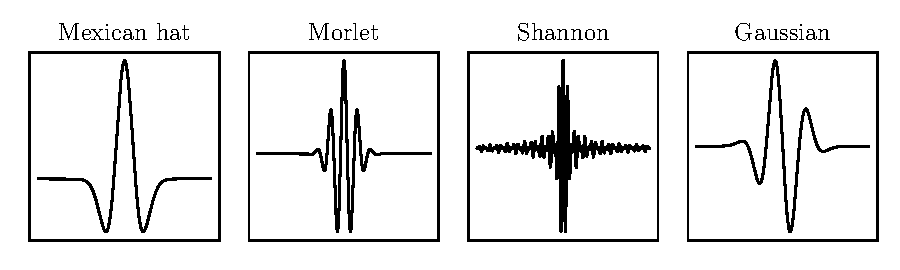
\includegraphics{figures/wavelets.pdf}
    \caption{Les différents types d'ondelettes}
    \label{fig:wavelets}
\end{figure}

\subsubsection{Transformée en ondelettes continue}
Mathématiquement, la transformation en ondelettes continue est définie par l'équation \ref{equation:cwt}:

\begin{equation}
    CWT_x^\psi(\tau, s)=\frac{1}{\sqrt{|s|}}\int_{-\infty}^{\infty}x(t)\psi^* \left(\frac{t-\tau}{s}\right)dt
    \label{equation:cwt}
\end{equation}

Où $x(t)$ est le signal original, $\psi^*$ est une fonction appelée \textbf{l'ondelette mère} ; $s$ et $\tau$ sont les facteurs de \textbf{dilatation} et \textbf{translation} respectivement. Le signal original est multiplié par l'ondelette mère qui est mise à l'échelle en utilisant différents facteurs de dilatation puis translatée sur le signal.

La sortie de \acrshort{cwt} est un scaleogram comme celui de la figure \ref{fig:scaleogram} qui est un scaleogram (tracé de contour rempli) de données de vibrations sur une durée de 25ms :

\begin{figure}[H]
    \centering
    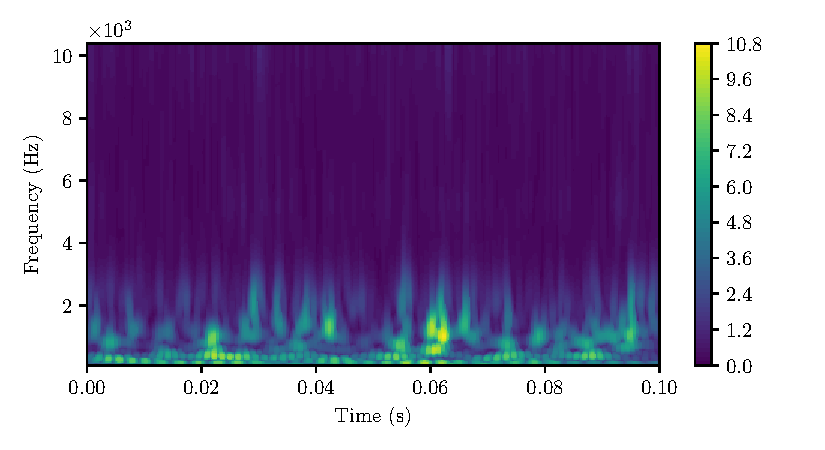
\includegraphics{figures/scaleogram.pdf}
    \caption{Scaleogram d'un échantillon de vibrations}
    \label{fig:scaleogram}
\end{figure}

Les axes x et y représentent respectivement le temps et la fréquence. Les différentes couleurs indiquent la hauteur (c'est-à-dire l'amplitude) de chaque fréquence (axe des y) à chaque instant-de-temps (axe des x), ce qui—différemment de la transformation de Fourier—fournit des informations sur les fréquences présentes dans le signal ainsi que sur les moments où ces fréquences sont présentes.

\subsubsection{Transformation en ondelettes discrète}%
\label{subsub:transformation_en_ondelettes_discrete}

Dans des applications pratiques, la transformation en ondelettes discrètes (\acrlong{dwt}: \acrshort{dwt}) est implémentée comme une banque de filtres où le signal est passé à travers des filtres passe-bas et passe-haut pour obtenir des \textbf{approximation} et des \textbf{coefficients de décomposition}. La figure \ref{fig:dwt} montre un \acrshort{dwt} avec 2 niveaux de décomposition qui donne des coefficients d'approximation et de décomposition du 2ème ordre :

\begin{figure}[H]
    \centering
    \begin{tikzpicture}[cell/.style={rectangle,draw, thick,align=center, minimum size=2em,inner sep=5pt}, input/.style={->}]

\node[cell] at (0,0) (xn) {$x[n]$};

\node[cell] at (-1.5,-1.5) (lpf1) {$LPF$};
\node[cell] at (1.5,-1.5) (hpf1){$HPF$};

\node[cell] at (-1.5,-3) (A1) {A1};
\node[cell, below = 1em of hpf1]  (D1) {D1};

\node[cell, below left = 2em of A1] (lpf2) {$LPF$};
\node[cell, below right = 2em of A1] (hpf2){$HPF$};

\node[cell, below = 1em of lpf2]  (A2) {A2};
\node[cell, below = 1em of hpf2]  (D2) {D2};

\draw[->, >=angle 60] (xn) -- ++(0,-1em) -- ++(0,-0.75em) -| (lpf1);
\draw[->, >=angle 60] (xn) -- ++(0,-1em) -- ++(0,-0.75em) -| (hpf1);

\draw[->, >=angle 60] (lpf1) -- (A1);
\draw[->, >=angle 60] (hpf1) -- (D1);

\draw[->, >=angle 60] (A1) -- ++(0,-1em) -- ++(0,-0.8em) -| (lpf2);
\draw[->, >=angle 60] (A1) -- ++(0,-1em) -- ++(0,-0.8em) -| (hpf2);

\draw[->, >=angle 60] (lpf2) -- (A2);
\draw[->, >=angle 60] (hpf2) -- (D2);

\node[] at (3,-0.9) (coord1) {};
\node[] at (3,-3.25) (coord2) {};

\end{tikzpicture}
    \caption{Transformation en ondelettes discrètes (\acrshort{dwt}) comme banque de filtres}
    \label{fig:dwt}
\end{figure}

\acrshort{dwt} donne deux séries de coefficients : \textbf{coefficients d'approximation} associé au filtre passe-bas et \textbf{coefficients de détail} associé au filtre passe-haut du \acrshort{dwt}. En appliquant à nouveau le \acrshort{dwt} sur les coefficients d'approximation, le niveau de décomposition suivant peut être obtenu. À chaque niveau, le signal original est sous-échantillonné d'un facteur 2, ce qui impose une limitation du nombre possible de niveaux de décomposition pour un signal donné.

\begin{figure}[h]
    \centering
    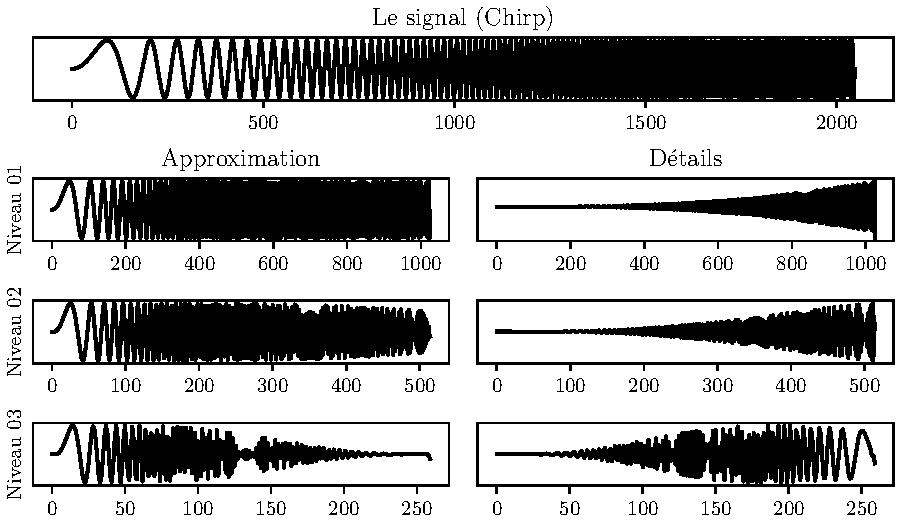
\includegraphics{figures/dwt_chirp_fr.pdf}
    \caption{Décomposition du signal de niveau 3 à l'aide de \acrshort{dwt}}
    \label{fig:dwt-chirp-signal}
\end{figure}



\subsection{Reduction de la dimensionalité}
\label{section:dimensionality-reduction}
La réduction de la dimensionnalité se réfère au processus consistant à prendre des données à haute dimension et à trouver une bonne représentation de ces données dans une dimension inférieure tout en préservant ses caractéristiques originales. La réduction de la dimensionnalité est effectuée pour l'extraction de caractéristiques en trouvant les principales composantes ou pour la visualisation (en réduisant le nombre de dimensions à 2 ou 3).
Il existe de nombreuses techniques et algorithmes de réduction de la dimensionnalité comme:
\begin{itemize}
    \item Principal Component Analysis (PCA)
    \item Autoencoders
    \item t-Distributed Stochastic Neighbor Embedding (t-SNE)
\end{itemize}

Il faut noter que pour les pronostics, où les données utilisées consistent en des entrées de capteurs où chaque variable a une signification physique et une interprétation directe, le fait d'effectuer une réduction de la dimensionnalité donnera les principales composantes, mais les nouvelles variables \textit{perdront leur interprétabilité physique} et \textit{devront être traitées comme des abstractions}.


\section{Diagnostic}
Le diagnostic se résume à un processus d'identification et de détermination de la relation entre les informations obtenues dans l'espace de mesure et les modes de défaillance des machines dans l'espace de défaillance. Le diagnostic comporte trois grandes étapes, à savoir la détection des défauts, l'isolation des défauts et l'identification des défauts. La détection des défauts est une tâche qui consiste à indiquer si un défaut a s'est déjà produite dans les machines surveillées. L'isolation des défauts consiste à trouver la composante de la défaillance et la position de la défaillance. L'identification des défauts est la dernière étape du diagnostic, qui tente de déterminer le mode et la gravité de la défaillance. Les trois étapes sont en corrélation entre eux. Cette dernière étape repose sur les résultats de la première et ne peut donc pas être réalisée individuellement \cite{Lei2016b}.

\section{Pronostic}
%TODO: translate
Le diagnostic est l'analyse de l'événement postérieur et le pronostic est l'analyse de l'événement antérieur. Le pronostic est beaucoup plus efficace que le diagnostic pour obtenir des performances sans arrêt de production. Le diagnostic est toutefois nécessaire lorsque la prédiction des erreurs de pronostic échoue et qu'une erreur se produit \cite{Jardine2006}.
Prognostics are the forecast or prediction of the future performance of a system, this prediction is based on its current state. The prediction is performed using a model, types of prognostics models are already discussed in details in section \ref{section:prognostics-approaches} but the focus of this current discussion is geared towards data-driven models. More concretely, what these models predict is the remaining useful life (\acrshort{rul}) defined in section \ref{section:rul-estimation}. Prognostics models—by estimating \acrshort{rul}—aim at scheduling maintenance actions according to the predictions and production constraints associated with the machine in order to achieve zero unscheduled equipment downtime.

\section{Décision de la maintenance}
La prochaine et dernière étape de toute approche pronostique consiste à utiliser les résultats du modèle développé (c'est-à-dire les prédictions ou les estimations pour le \acrshort{rul} du système) afin de réaliser des actions de maintenance préventive meilleures et plus précises. Les personnes chargées de la maintenance doivent analyser les résultats du modèle avant de prendre des mesures, car tout modèle comporte une erreur inhérente associée à ses prévisions. Habituellement, les modèles basés sur des données fournissent des intervalles de confiance associés à leurs prédictions qui doivent être considérés avec soin. Il convient également de noter que ces intervalles de confiance reflètent la certitude des modèles quant à leurs prédictions sur la base des données fournies pour l'entraînement. Dans les applications réelles, un nouveau mode de défaillance imprévu peut se produire, ce qui n'était peut-être pas le cas auparavant, et n'a donc pas été prévu pour le modèle dans les données utilisées pour le construire. Ceci est plus ou moins associé à la capacité de différents types de modèles à généraliser pour de nouvelles données imprévues, mais en général, il est bien connu que tout modèle d'entraînement sera moins fiable lorsqu'il effectue des prédictions en utilisant des données que le modèle ne voyait pas avant \cite{Chung2018}. C'est pourquoi il est essentiel de fournir des données de qualité qui reflètent différents modèles de dégradation et modes de défaillance pour que le modèle puisse faire des prédictions plus robustes et plus fiables.

\section{Conclusion}
L'élaboration d'un modèle de pronostic (fondé sur des données) est un processus qui nécessite de nombreuses étapes : de l'acquisition des données nécessaires à la construction du modèle à l'utilisation des prévisions du modèle pour prendre des décisions de maintenance meilleures et plus précises qui se traduisent par moins (voire zéro) de temps d'arrêt imprévu ; ceci réduit les coûts et diminue les pertes de production, ce dernier point étant le but ultime de toute cette discussion et de la littérature sur les pronostics/la maintenance préventive en général. Cette discussion se concentre sur les modèles basés sur les données, l'un des modèles qui a prouvé sa grande capacité à apprendre des modèles non linéaires complexes dans les données sont les réseaux de neurones. Ces modèles ont une architecture différente en fonction de la structure des données. Ils seront présentés et expliqués en détail dans le prochain chapitre.

\begin{comment}

\section{Décision de la maintenance}
The next and the last step of any prognostics approach is to use the output of the developed model (i.e. predictions, or estimations for the system's \acrshort{rul}) in making better and more accurate preventive maintenance actions. Maintenance decision makers should analyze the outputs of the model prior to taking any actions, since any model has an inherent error associated with its predictions. Usually, data-driven models provide confidence intervals associated with their predictions which must be considered carefully. Also it must be noted that those confidence itervals are reflection of the models certainty of its predictions based on the data provided for the training, in real applications a new unforeseen failure mode can occure which may not have happened before, thus it wasn't provided for the model as part of the data used to consutrct it. This is more or less associated with the ability of different types of models to generalize for new unforeseen data, but in general it is well-known fact that any data-driven model will be less reliable when performing predictions using data that the model didn't see before \cite{Chung2018}. That's why providing quality data that reflects different degradation patterns and fault modes is essential for the model to make more robust and reliable predictions.

\section{Conclusion}
Developing a (data-driven) prognostics model is a process that requires many steps: from data acquisition required to construct the model to employing the model predictions in making better and more accurate maintenance decisions which result in less (or even zero) unscheduled downtime this reduced costs and decreased production loss, the latter being the ultimate goal of all this discussion and prognostics/preventive maintenance literature in general. The focus of this discussion is data-driven models, one of the models that proved great ability in learning complex non-linear patterns in data are neural networks. These models have different architecture depending on the structure of data. They will be presented and explained in details in the next chapter.

\end{comment}
